\newpage

\section{Partie 1: Quelques opérations de base sur les signaux}

\subsection{Signal numérique de synthèse}

\subsubsection{Génération du signal}

Un signal sinusoïdal de fréquence \( f_0 \) est généré par la fonction suivante:

\[
x[n] = \sin\left(2\pi f_0 \frac{n}{f_e}\right)
\]

où \( f_e \) est la fréquence d’échantillonnage et \( N \) le nombre d’échantillons.

\begin{figure}[!h]
\centering
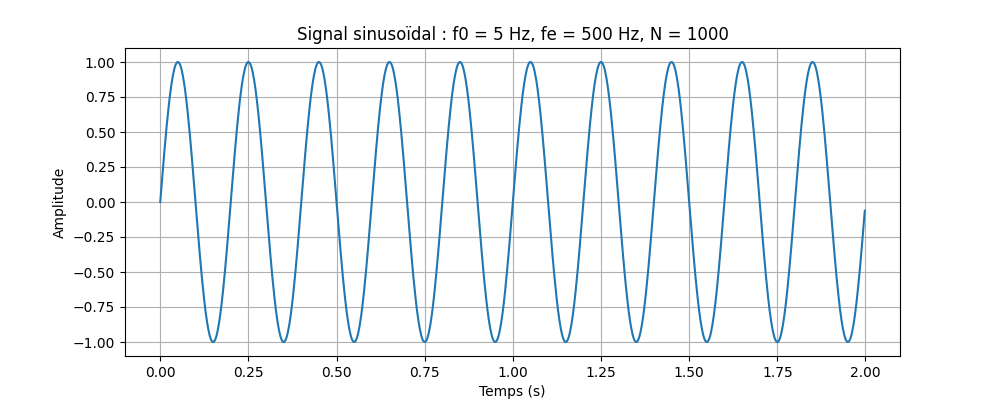
\includegraphics[width=17cm]{screenshots/signal_echantillone.png}
\caption{Signal sinusoïdal échantillonné}
\end{figure}

\subsubsection{Énergie et puissance}

L'énergie d’un signal discret \( x[n] \) est donnée par :

\[
E = \sum_{n=0}^{N-1} x[n]^2
\]

Et la puissance moyenne par :

\[
P = \frac{1}{N} \sum_{n=0}^{N-1} x[n]^2
\]

Considérons un signal sinusoïdal discret de la forme :
\[
x[n] = A \cdot \sin\left(2\pi f_0 \frac{n}{f_e} \right)
\]

La puissance moyenne théorique d’un signal périodique est calculée par la  formule:

\[
P = \lim_{N \to \infty} \frac{1}{N} \sum_{n=0}^{N-1} x[n]^2
\]

En utilisant l’identité trigonométrique :
\[
\sin^2(\theta) = \frac{1 - \cos(2\theta)}{2}
\]
on obtient :
\[
x[n]^2 = A^2 \cdot \frac{1 - \cos\left(4\pi f_0 \frac{n}{f_e} \right)}{2}
\]

Ainsi, la puissance devient :
\[
P = \lim_{N \to \infty} \frac{1}{N} \sum_{n=0}^{N-1} A^2 \cdot \frac{1 - \cos\left(4\pi f_0 \frac{n}{f_e} \right)}{2}
= \lim_{N \to \infty}  \frac{A^2}{2} - \frac{A^2}{2N} \sum_{n=0}^{N-1} \cos\left(4\pi f_0 \frac{n}{f_e} \right)
= \frac{A^2}{2}
\] 

Donc dans notre cas la puissance moyenne théorique est égale à 0.5.

Pour la puissance moyenne calculée numériquement pour le signal échantillonné on a la méme formule mais sans la limite:

\[
P = \frac{A^2}{2} - \frac{A^2}{2N} \sum_{n=0}^{N-1} \cos\left(4\pi f_0 \frac{n}{f_e} \right)
\] 

\textbf{Cas idéal :} si $N$ est un multiple entier de la période du signal (i.e., $N$ couvre un nombre entier de périodes), alors la somme des cosinus s’annule :
\[
\sum_{n=0}^{N-1} \cos\left(4\pi f_0 t \right) = 0 \quad \Rightarrow \quad P = \frac{A^2}{2}
\]

\textbf{Cas général :} si $N$ n’est pas un multiple exact de la période, la somme ne s’annule pas et on observe une légère déviation de la puissance par rapport à $\frac{A^2}{2}$. Cela est dû au fait que le signal est tronqué entre deux points non symétriques.\\

En variant N on trouve plusieurs valeurs de la puissance moyenne qui restent proches de la valeur théorique:

\begin{figure}[!h]
\centering
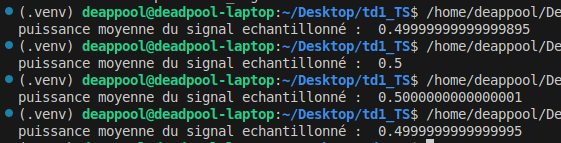
\includegraphics[width=15cm]{screenshots/puissance_et_energie.png}
\caption{Énergie et puissance du signal}
\end{figure}

\subsubsection{Quantification}

\begin{figure}[!h]
\centering
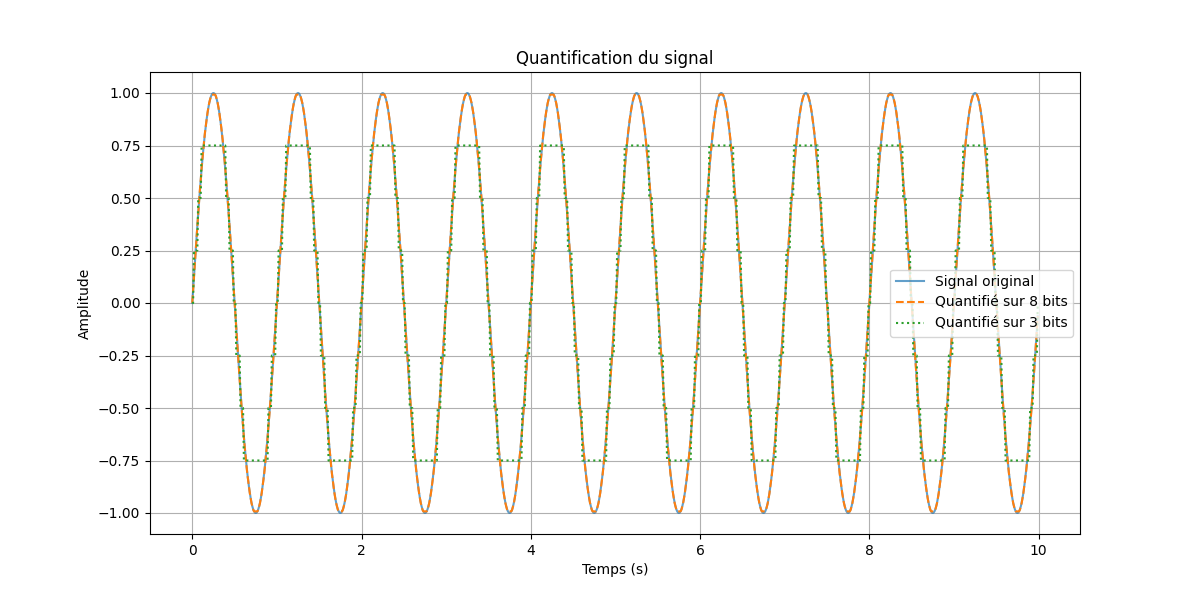
\includegraphics[width=15.5cm]{screenshots/quantification_graph.png}
\caption{Quantification du signal à 3 et 8 bits}
\end{figure}

Pour la quantification à 3 bits, on retrouve bien 8 niveaux de quantification.

\begin{figure}[!h]
\centering
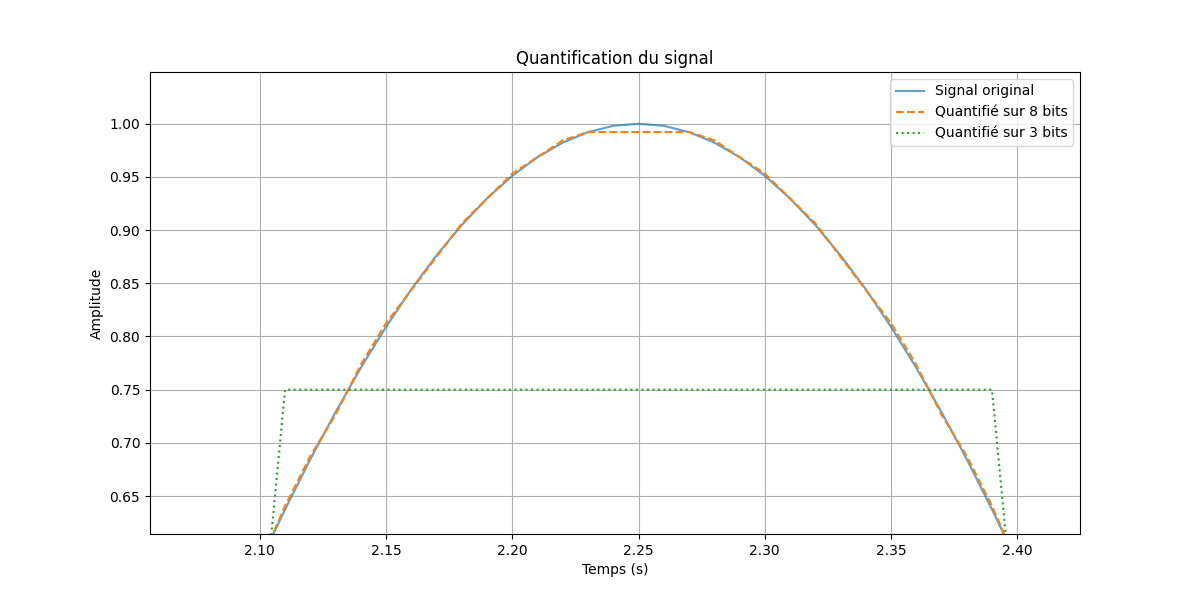
\includegraphics[width=17cm]{screenshots/quantification_graph_zoomed.png}
\caption{Zoom sur la quantification du signal à 3 et 8 bits}
\end{figure}

Le signal à 8 bits suit mieux la forme continue du signal d’origine mais on voit quand méme quelques erruers. À 3 bits, les marches sont plus visibles et le signal produit est significativement moins fidéle au signal d'origine.\\

\textbf{SNR (Signal-to-Noise Ratio)} :

\[
\text{SNR} = 10 \log_{10} \left(\frac{E_{\text{signal}}}{E_{\text{bruit}}} \right)
\]

\begin{figure}[!h]
\centering
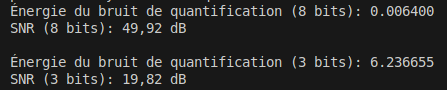
\includegraphics{screenshots/snr_quantification.png}
\caption{SNR pour chaque niveau de quantification}
\end{figure}

On remarque que l'energie du bruit est plus élevée pour le signal quantifié à 3 bits. Le résultat est logique
car on voit sur le graphe que ce signal est plus éloigné du signal d'origine comparé au signal quantifié à 8 bits.
On a la méme conclusion en raisonant sur le SNR: SNRq8 > SNRq3.

\subsection{Signal audio}

\subsubsection{Enregistrement}

Les mots « Bonjour » et « ChatGpt » ont été enregistrés via Audacity (voir figure \ref{fig:signal_enregistre}).

\subsubsection{Restitution à différentes fréquences}

L’audio est lu à \( f_e \), \( 2 f_e \) et \( \frac{f_e}{2} \). 

\textbf{Effets observés} :

\begin{itemize}
    \item \textbf{Durée :} doubler la fréquence de restitution divise la durée par deux (voix accélérée), tandis que la diviser par deux double la durée (voix ralentie).
    \item \textbf{Hauteur :} multiplier la fréquence de restitution rend la voix plus aiguë (fréquences doublées), la diminuer la rend plus grave (fréquences divisées).
\end{itemize}

Lorsque la fréquence de restitution est trop grande ou trop petite comparée à la fréquence d’échantillonnage, le son devient incompréhensible. Le son est trop rapide ou trop lent, mais aussi on ne reconnaît plus les mots. Cela s'explique notamment par le déplacement des formants, c’est-à-dire des pics de résonance caractéristiques des voyelles et consonnes, qui changent de position dans le spectre. Leur modification rend la parole méconnaissable, car ce sont eux qui permettent d’identifier les sons du langage.

\subsubsection{Quantification du signal audio}

\begin{itemize}
    \item À 3 bits : le son devient rugueux et très bruité, fortement altéré.
    \item À 8 bits : la voix reste compréhensible mais moins naturelle.
\end{itemize}

\subsubsection{Extraction et séparation de mots}

Après repérage visuel, les deux mots ont été extraits via tranches temporelles.


\begin{figure}[!h]
\centering
\includegraphics[width=10cm]{screenshots/signal_enregistré.png}
\caption{Signal audio enregistré}
\label{fig:signal_enregistre}
\end{figure}

\begin{figure}[h]
\centering
\begin{subfigure}[b]{0.45\textwidth}
    \centering
    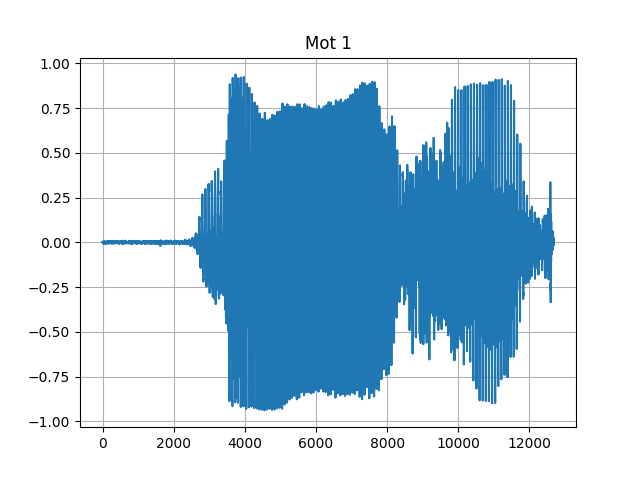
\includegraphics[width=9cm]{screenshots/mot1_graphe.png}
    \caption{Mot 1: "Bonjour"}
\end{subfigure}
\hfill
\begin{subfigure}[b]{0.45\textwidth}
    \centering
    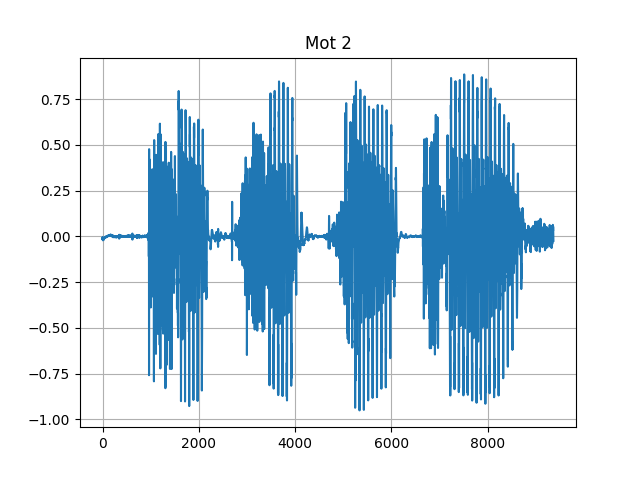
\includegraphics[width=9cm]{screenshots/mot2_graphe.png}
    \caption{Mot 2: "ChatGpt"}
\end{subfigure}
\caption{Séparation des mots dans le signal audio}
\end{figure}

\section{Partie 2: Classification des signaux}

\subsection{Exemple de calcul théorique}

Soit un signal sinusoïdal discret défini par :
\[
x[n] = A \sin(2\pi f n T_e)
\]

L'autocorrélation théorique du signal discret est définie par :
\[
R_{xx}[k] = \lim_{N \to \infty} \frac{1}{N} \sum_{n=0}^{N-1} x[n] \cdot x[n+k]
\]

En remplaçant l’expression de \( x[n] \) :
\[
R_{xx}[k] = \lim_{N \to \infty} \frac{1}{N} \sum_{n=0}^{N-1} A \sin(2\pi f n T_e) \cdot A \sin(2\pi f (n + k) T_e)
\]

\[
= A^2 \cdot \lim_{N \to \infty} \frac{1}{N} \sum_{n=0}^{N-1} \sin(2\pi f n T_e) \cdot \sin(2\pi f n T_e + 2\pi f k T_e)
\]

En utilisant l'identité trigonométrique :
\[
\sin(a)\sin(b) = \frac{1}{2} [\cos(a - b) - \cos(a + b)]
\]

On a :
\[
\sin(2\pi f n T_e) \cdot \sin(2\pi f n T_e + 2\pi f k T_e) = \frac{1}{2} \left[ \cos(2\pi f k T_e) - \cos(4\pi f n T_e + 2\pi f k T_e) \right]
\]

\[
\Rightarrow R_{xx}[k] = \frac{A^2}{2} \cos(2\pi f k T_e)
\]

car la somme de \( \cos(4\pi f n T_e + \cdot) \) sur une grande fenêtre \( N \) tend vers 0.

\textbf{Conclusion :} l'autocorrélation théorique du signal sinusoïdal discret est donnée par :
\[
\boxed{R_{xx}[k] = \frac{A^2}{2} \cos(2\pi f k T_e)}
\]

où :
\begin{itemize}
  \item \( A \) est l’amplitude du signal,
  \item \( f \) est la fréquence du signal en Hz,
  \item \( T_e = \frac{1}{f_e} \) est la période d’échantillonnage,
  \item \( k \in \mathbb{Z} \) est le décalage (lag) discret.
\end{itemize}

\subsection{Programmation}

On calcule l'autocorrélation pour un signal sinusoïdal échantillonné en utilisant la formule : 
\[
R_{xx}[k] = \frac{1}{N} \sum_{n=0}^{N-1} x[n] \cdot x[n+k]
\]

\begin{lstlisting}[language=Python]
    def autocorrelation_manual(x):
    N = len(x)
    r = np.zeros(2*N - 1)
    lags = np.arange(-N + 1, N)
    for k in range(-N + 1, N):
        somme = 0
        for n in range(N - abs(k)):
            somme += x[n] * x[n + k] if k >= 0 else x[n - k] * x[n]
        r[k + N - 1] = somme
    return lags, r
\end{lstlisting}

On compare avec l'autocorrelation calculée avec numpy et on trace la différence entre les deux résultats pour visualiser les écarts.
Pour convertir les abcisses en secondes, on utilise la formule :  
\[ \text{t} = {\text{k}}.{T_e} = \frac{\text{k}}{f_e} \]

\begin{figure}[!h]
\centering
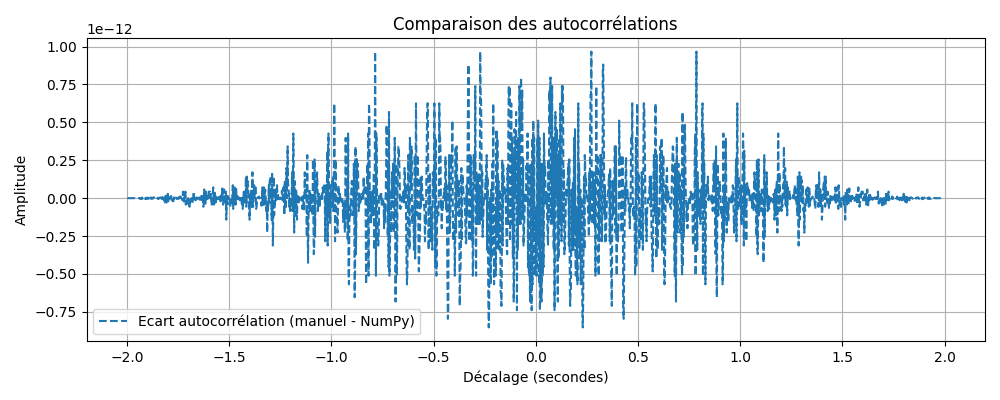
\includegraphics[width=17cm]{screenshots/ecart_autocorrelation.png}
\caption{Ecart entre l'autocorrélation manuelle et celle de numpy}
\end{figure} 

L'ecart est trop petit entre les deux méthodes (de l'ordre de \(10^{-12}\)). Ceci est dû à la précision numérique des calculs et au fait que l'autocorrelation numpy est calculée différemment en utilisant plusieurs techniques d'optimisation.\\

On calcule le rapport des énergies entre la différence entre les deux méthodes et l'autocorrelation de numpy:
\[ \text{rapport} = \frac{\sum_{k=0}^{N-1} \text{diff}[k]^2}{\sum_{k=0}^{N-1} \text{autocorr}[k]^2} \] \\

On trouve plusieurs valeurs de rapport pour différentes valeurs de N. Ceci est dû à la variation de l'énergie du signal en fonction de N, car l'autocorrelation et l'énergie sont sensibles à la longueur du signal (somme de 0 à N-1). On rajoute donc des valeurs au numérateur et au dénominateur dans le calcul de ce rapport (qui ne sont pas équivalentes vu l'écart entre les deux méthodes) ce qui expliques des valeurs de rapport différentes.

\begin{figure}[!h]
\centering
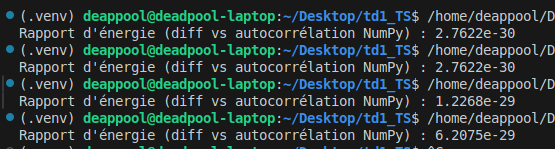
\includegraphics[width=15cm]{screenshots/valeur_rapport.png}
\caption{Valeurs du rapport pour plusieurs valeurs de N}
\end{figure} 

\subsection{Application à la classification de quelques signaux simples}

On génére les signaux demandés avec le code suivant :
\newpage
\begin{lstlisting}[language=Python]
# Parametres communs
fe = 11000          # frequence d'echantillonnage
duration = 1     # duree en secondes
t = np.linspace(0, duration, int(fe * duration), endpoint=False)

# 1. Signal sinusoidal de 200 Hz
f = 200
sinus = np.sin(2 * np.pi * f * t)

# 2. Signal triangulaire centre en 0 (serie de Fourier avec 10 termes)
tri = np.zeros_like(t)
for k in range(1, 11):
    n = 2 * k - 1  # uniquement les harmoniques impaires
    tri += ((-1)**((k+1)) / n**2) * np.sin(2 * np.pi * n * f * t)
tri *= (8 / (np.pi**2))  # normalisation serie de Fourier

# 3. Bruit blanc gaussien
taille = fe  # 1 seconde
bruit = np.random.randn(taille)
bruit /= np.max(np.abs(bruit))  # normalisation pour eviter la saturation
\end{lstlisting}

\begin{figure}[!h]
\centering
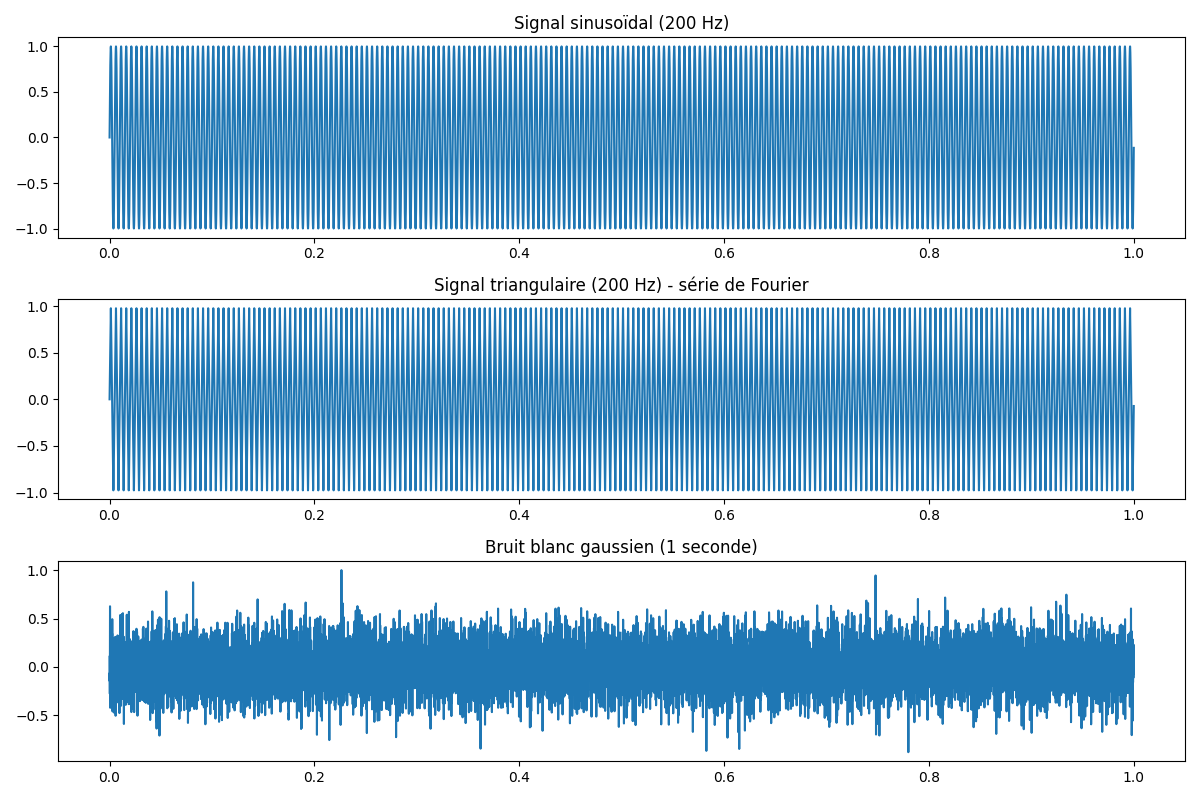
\includegraphics[width=17cm]{screenshots/generation_signaux.png}
\caption{Signaux générés}
\end{figure} 

\begin{figure}[!h]
\centering
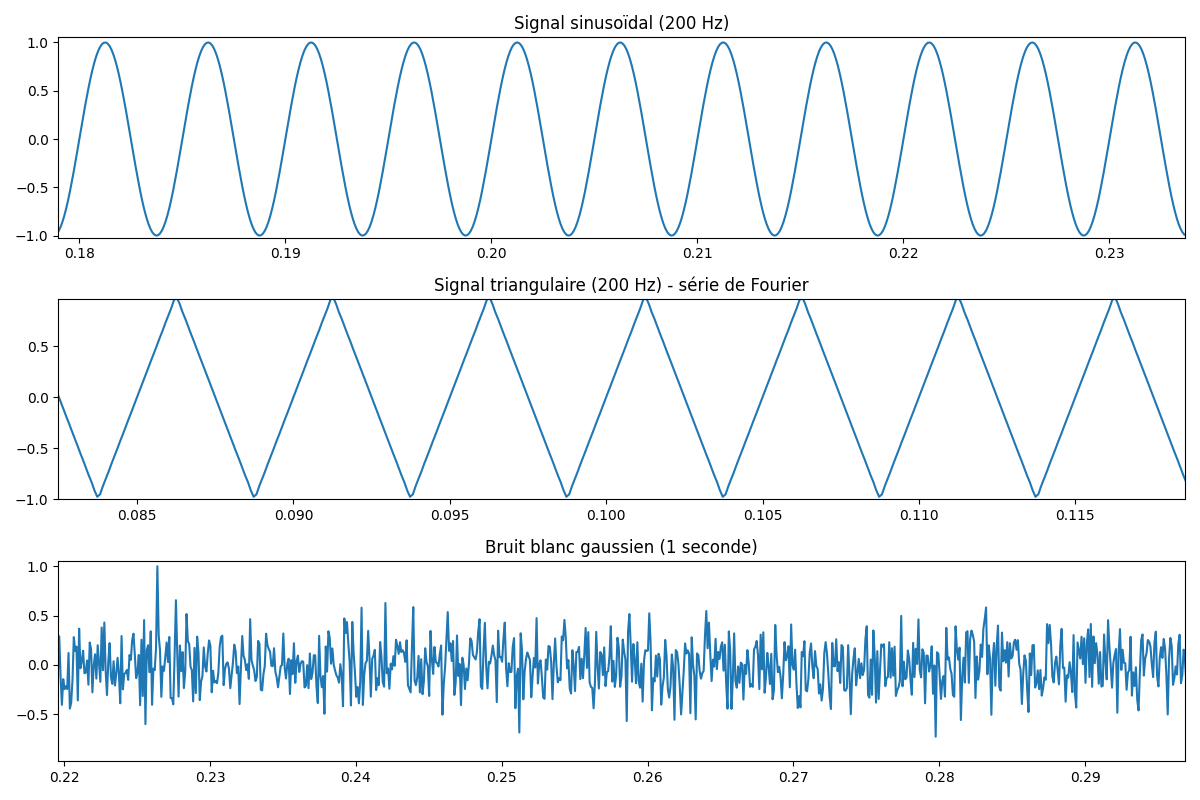
\includegraphics[width=17cm]{screenshots/generation_signaux_zoom.png}
\caption{Signaux générés (zoom)} 
\end{figure} 

\newpage

On calcule l'autocorrélation pour chaque signal sur une partie de durée de 30ms. C’est une durée typique en traitement du signal pour analyser la parole (équilibre entre résolution temporelle et fréquence). Elle est suffisante pour voir une structure (formants, périodicité...) sans mélanger des parties trop différentes du signal. On trace également l'autocorrélation du signal enregistré sur deux tranches de 30ms (et 80ms) à des moments différents (1000ms et 1500ms). Cela nous permettera de de comparer l'autocorrélation à différents moments afin de mettre en oeuvre la non-stationnarité du signal.\\

Un signal est dit \textbf{stationnaire} si ses propriétés statistiques, telles que la moyenne, la variance et l'autocorrélation, ne varient pas dans le temps.\\

L'analyse des autocorrélations montre que :
\begin{itemize}
    \item Le signal vocal « aa » est \textbf{non stationnaire} car ses caractéristiques changent entre différentes tranches temporelles (voix humaine évolue dans le temps).
    \item Le signal de bruit blanc gaussien est \textbf{stationnaire}, ses propriétés statistiques étant constantes dans le temps (Pic au centre, décroissance rapide).
    \item Les signaux sinusoïdal et triangulaire, synthétisés sur quelques périodes, sont également \textbf{stationnaires} car ils sont périodiques et leurs statistiques ne varient pas dans le temps.
\end{itemize}

\begin{figure}[!h]
\centering
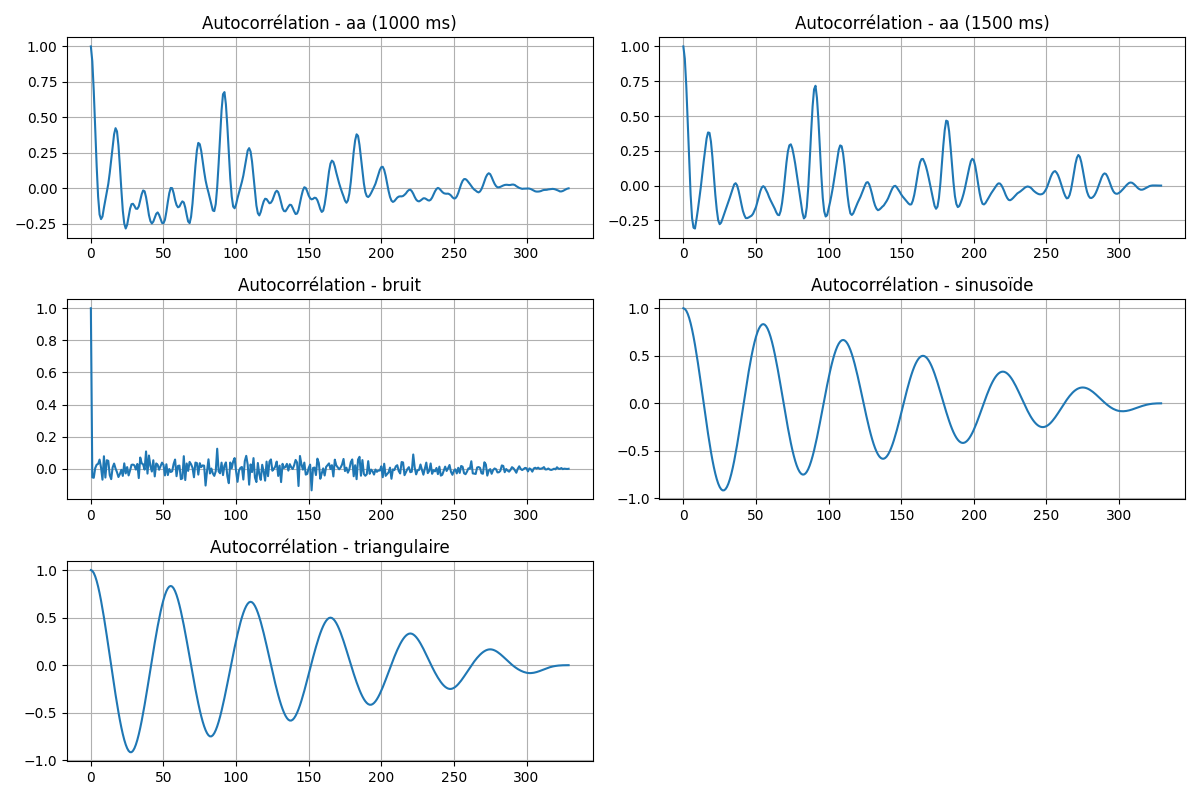
\includegraphics[width=17cm]{screenshots/autocorr_signaux_30ms.png}
\caption{autocorrélation des signaux sur 30ms} 
\end{figure} 

\begin{figure}[!h]
\centering
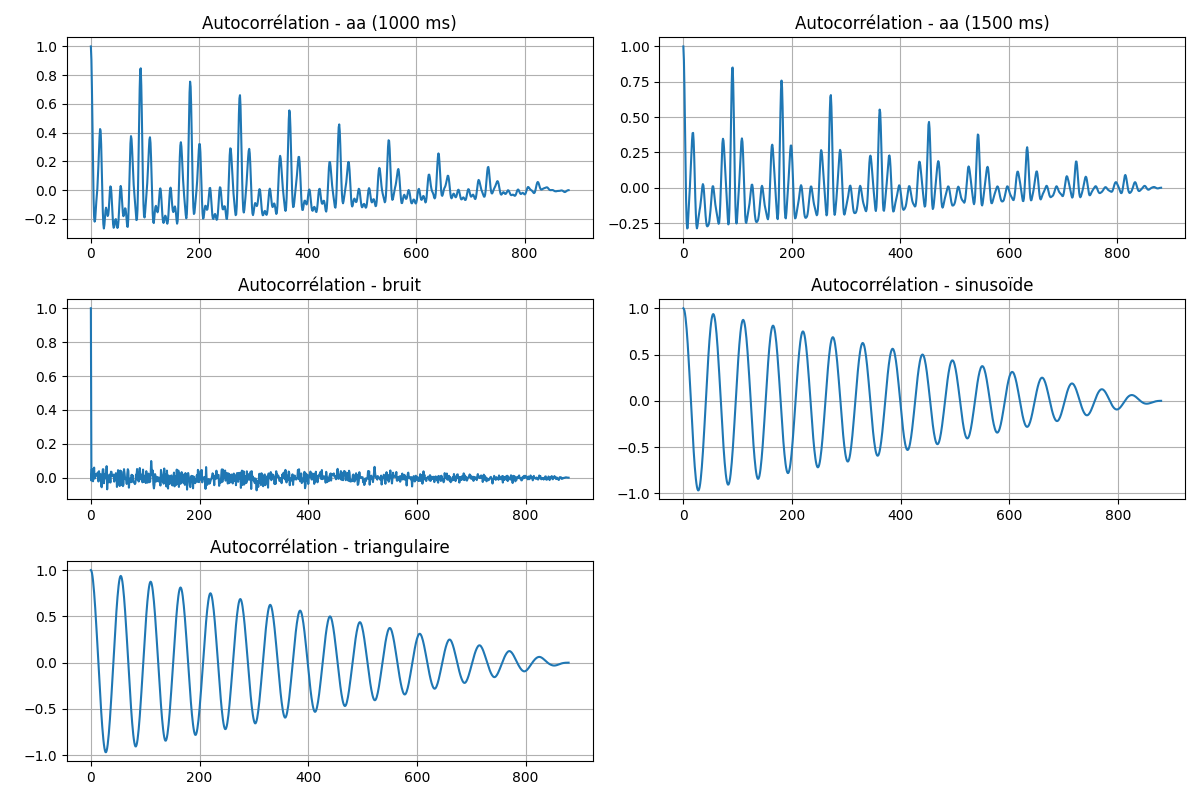
\includegraphics[width=17cm]{screenshots/autocorr_signaux_80ms.png}
\caption{autocorrélation des signaux sur 80ms} 
\end{figure}

\newpage
\subsection{Classification de signaux de parole voisés ou non voisés}

Le signal est découpé en tranches de 30 ms pour analyser leur autocorrélation. Les résultats montrent clairement deux types de comportements :

\begin{itemize}
    \item \textbf{Parties non voisées} (« chhhhh ») : l'autocorrélation est bruitée, sans périodicité marquée, caractéristique des sons fricatifs.
    \item \textbf{Parties voisées} (« aaaa ») : l'autocorrélation présente des pics réguliers, révélant une structure périodique due à la vibration des cordes vocales.
\end{itemize}

\begin{figure}[h!]
    \centering
    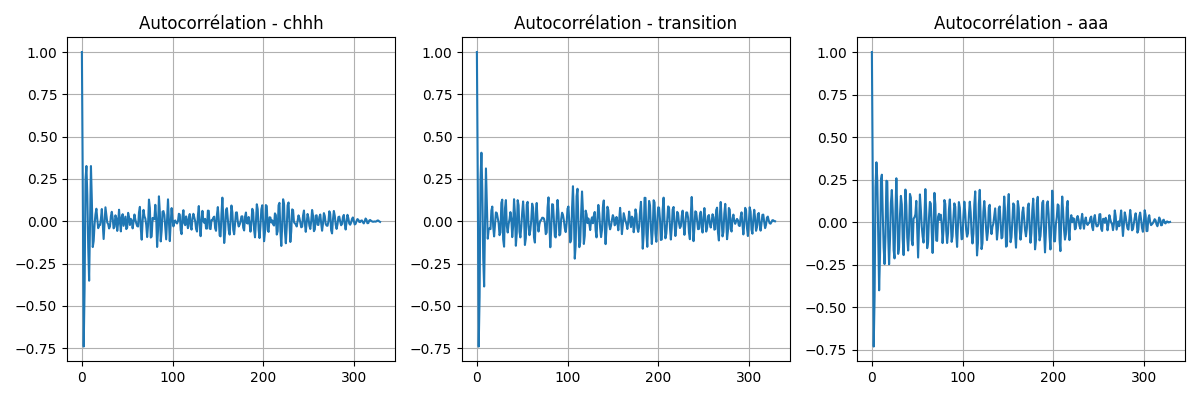
\includegraphics[width=17cm]{screenshots/autocorrelation_chat_2.png}
    \caption{Autocorrélation de différentes tranches du mot « chat » : (gauche) non voisée, (milieu) transition, (droite) voisée.}
\end{figure}


L’autocorrélation permets d'estimer la fréquence fondamentale \(f_0\) d’un signal voisé. On s’attend à ce qu’un signal périodique présente un maximum secondaire au retard correspondant à sa période fondamentale \(T_0 = \frac{1}{f_0}\).\\

Pour identifier les pics secondaires dans l’autocorrélation, nous utilisons la fonction \verb|find_peaks| de \texttt{scipy.signal}.
Afin d’éviter de détecter des pics non significatifs dus au bruit ou à des résonances (formants), le paramètre \textbf{height} qui correspond à la hauteur minimale doit être soigneusement choisis pour ignorer les pics trop faibles dus au bruit. Nous avons fixé ce seuil à 0{,}3 après normalisation.\\

Pour la tranche correspondant à la voyelle \textit{« a »} dans l’enregistrement (partie voisée), nous obtenons après traitement:

\begin{itemize}
    \item Indices du premier pic détecté : 133
    \item On en déduit une fréquence fondamentale :
    \[
    f_0 = \frac{f_e}{\text{lag}} = \frac{16\,000}{133} \approx 120{,}3\ \mathrm{Hz}
    \]
\end{itemize}

Ce résultat est conforme aux plages typiques pour une voix masculine (85–180 Hz). 
Il est important de noter que la fréquence fondamentale ne caractérise pas la voyelle elle-même, mais le locuteur.


\newpage
\section{Partie 3: Aspects fréquentiels}
\subsection{Echantillonnage}


Le théorème de Nyquist-Shannon stipule qu’un signal bande limitée, dont la fréquence maximale est $f_0$, peut être parfaitement reconstruit à partir de ses échantillons si la fréquence d’échantillonnage vérifie :
\[
f_e > 2 f_0
\]
La fréquence $f_e = 2 f_0$ est appelée \textbf{fréquence de Nyquist} et constitue la limite minimale pour éviter le phénomène de repliement spectral (\textit{aliasing}).

On échantillone donc le signal selon trois cas distincts :

\begin{itemize}
    \item \textbf{Cas 1 :} $f_e = 2f_0$ (fréquence de Nyquist),
    \item \textbf{Cas 2 :} $f_e = 5f_0$ (fréquence supérieure),
    \item \textbf{Cas 3 :} $f_e = 0{,}8f_0$ (fréquence inférieure).
\end{itemize}

On vois que pour les deux premiers cas, le signal échantillonné est fidèle à la forme du signal d’origine. En revanche, pour le troisième cas, l’échantillonnage à une fréquence inférieure à la fréquence de Nyquist entraîne un repliement spectral, rendant le signal méconnaissable.
\begin{figure}[h!]
    \centering
    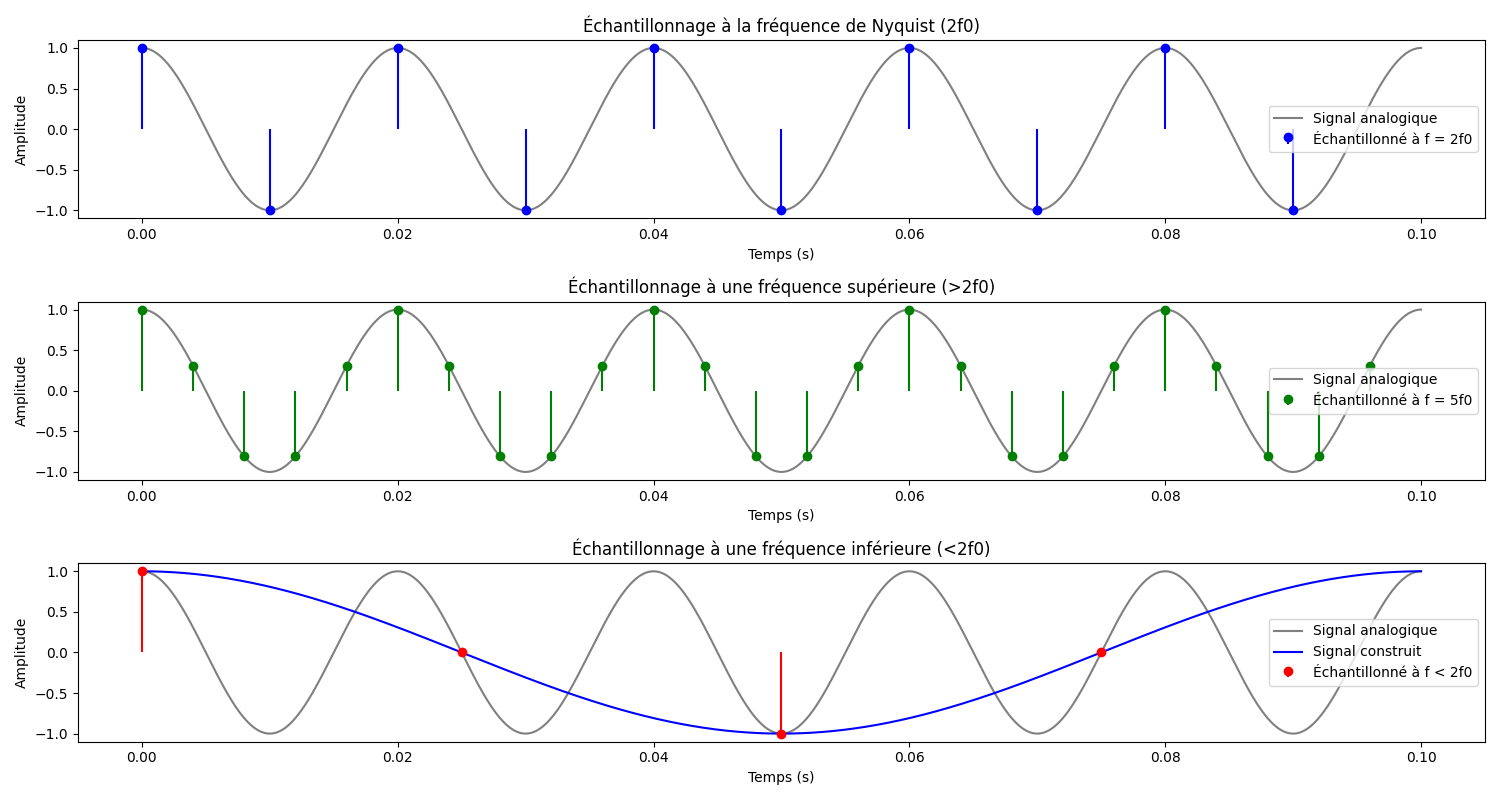
\includegraphics[width=17cm]{screenshots/echantillonage_partie3.png}
    \caption{Signaux échantillonnés}
\end{figure}

\subsection{La Transformée de Fourier discrète (TFD)}

Nous avons implémenté une fonction en \texttt{Python} permettant de calculer et tracer la densité spectrale d’énergie d’un signal extrait d’un fichier \texttt{.wav}. La fonction lit le fichier audio, extrait une tranche du signal à partir d’un indice donné, applique une fenêtre de Hanning pour atténuer les effets de bord, puis calcule la transformée de Fourier rapide (\texttt{FFT}) sur $2^n$ points. La densité spectrale est obtenue en prenant le module au carré des coefficients de la FFT (représentant l’énergie en fréquence), normalisée et convertie en décibels (dB) selon la formule :
\[
P_{\mathrm{dB}}(f) = 10 \log_{10} \left( \frac{|\mathrm{FFT}(f)|^2}{\max(|\mathrm{FFT}(f)|^2)} + \varepsilon \right),
\] \\

avec $\varepsilon$ un terme petit ($10^{-12}$) pour éviter les problèmes numériques liés au logarithme de zéro.\\

La courbe obtenue est symétrique par rapport à l’axe des fréquences, car la FFT calcule les coefficients complexes pour les fréquences positives et négatives. On ne garde que la moitié positive du spectre.\\

Le choix de $2^n$ (taille de la FFT) influence la **résolution fréquentielle**. Plus $n$ est grand, plus les fréquences sont discrétisées finement, ce qui permet de mieux isoler les pics correspondant aux composantes harmoniques du signal.

\begin{figure}[h!]
    \centering
    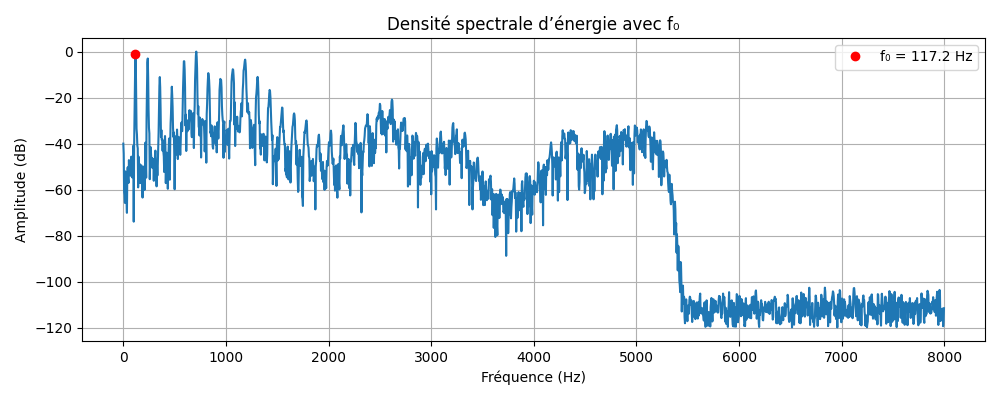
\includegraphics[width=17cm]{screenshots/fft_detection_f0.png}
    \caption{FFT}
\end{figure}


Sur le spectre obtenu, on observe une structure en pics caractéristiques d’un signal périodique voisé (ici le phonème \textit{aaa}). La fréquence fondamentale correspond au premier pic significatif au-dessus du bruit. À partir du spectre, nous détectons une fréquence fondamentale de \textbf{117{,}2 Hz}.\\

Ce résultat est très proche de celui obtenu par l’autocorrélation dans le domaine temporel, où nous avions trouvé une fréquence de \textbf{120{,}3 Hz} (3.1 Hz de différence). Cette légère différence peut s’expliquer par :
\begin{itemize}
    \item la résolution fréquentielle limitée de la FFT (dépendante de la taille de la tranche),
    \item les effets de la fenêtre de Hanning qui modifie légèrement le contenu fréquentiel,
    \item et les arrondis ou approximations dans la localisation du pic.
\end{itemize}
Malgré cela, les deux méthodes convergent vers une estimation très cohérente de la fréquence fondamentale, typique d’une voix d’homme (comprise entre 85 et 180 Hz).\\

Le \emph{zero-padding} consiste à compléter un signal par des zéros à la fin. Cette opération n’ajoute aucune nouvelle information, mais elle permet d’augmenter artificiellement la longueur du signal, ce qui améliore la **résolution fréquentielle** du spectre après transformation de Fourier.

Nous avons implémenté une fonction \texttt{zero\_padding} en \texttt{Python}, prenant en entrée le signal initial et le nombre de zéros à ajouter, et renvoyant le signal étendu.

\begin{lstlisting}[language=Python]
    def zero_padding(signal, nb_zeros):
    return np.hstack((signal, np.zeros(nb_zeros)))
\end{lstlisting}

Nous avons ensuite comparé les densités spectrales d’énergie (obtenues par FFT) avant et après zero-padding.

Le résultat montre que :
\begin{itemize}
  \item les **positions des pics** dans le spectre restent inchangées (le contenu fréquentiel est le même),
  \item mais les courbes sont **plus lisses** comme on peut le voir dans la figure \ref{fig:fft_zero_padding_zoom} et les pics **mieux localisés** après padding, ce qui facilite l’estimation des fréquences fondamentales,
  \item le zero-padding agit donc comme une **interpolation en fréquence**.
\end{itemize}

Cela est particulièrement utile pour distinguer des pics proches ou évaluer plus précisément une fréquence fondamentale.

\begin{figure}[h!]
    \centering
    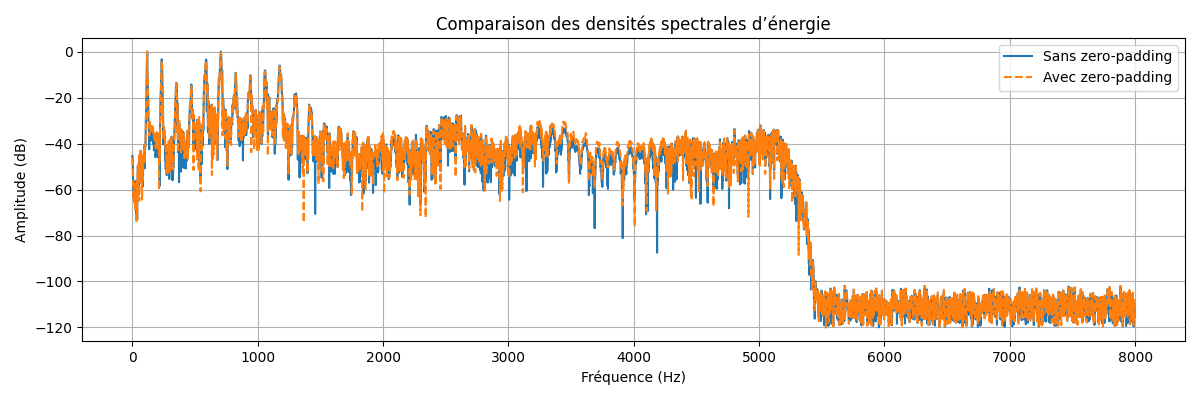
\includegraphics[width=17cm]{screenshots/fft_avec_zero_padding.png}
    \caption{FFT avec et sans zero-padding}
\end{figure}

\begin{figure}[h!]
    \centering
    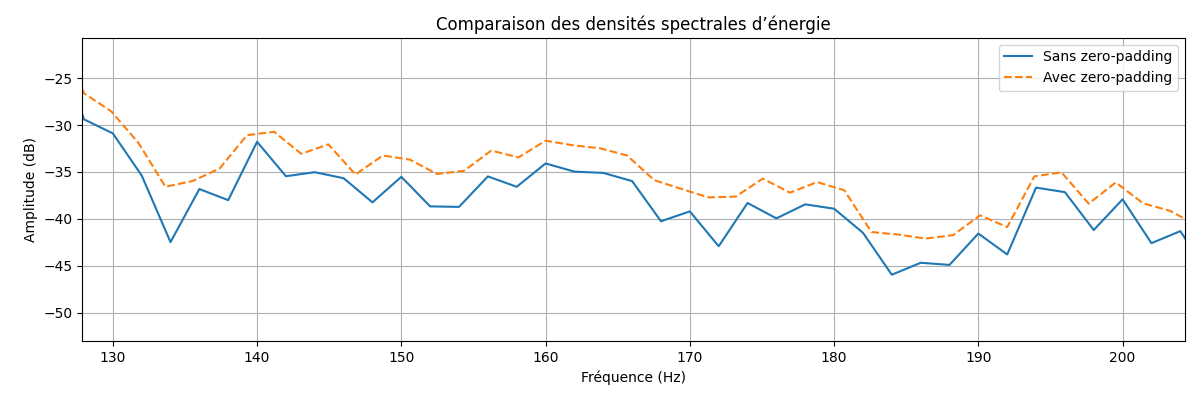
\includegraphics[width=17cm]{screenshots/fft_avec_zero_padding_zoom.png}
    \caption{FFT avec et sans zero-padding (zoom)}
    \label{fig:fft_zero_padding_zoom}
\end{figure}

\newpage
On peut faire directement du zero-padding dans la fonction \textbf{np.fft.fft(x, n)}.

\begin{itemize}
    \item Si \( n \) est supérieur à la longueur de \( x \), la fonction ajoute des zéros à la fin de \( x \) jusqu'à atteindre la longueur \( n \).
    \item Si \( n \) est inférieur ou égal à la longueur de \( x \), la fonction tronque \( x \) à la longueur \( n \).
\end{itemize}

\subsection{Changement de fréquence d’échantillonnage}

Il est essentiel de bien distinguer deux opérations proches mais conceptuellement différentes :

\begin{itemize}
    \item \textbf{Changer la cadence (changer la vitesse de lecture)} consiste à lire un signal audio plus vite ou plus lentement, sans modifier son contenu en échantillons. Cela revient à modifier la \textit{fréquence d’échantillonnage effective} sans changer les données elles-mêmes. Par exemple :
    \begin{itemize}
        \item Lire un signal échantillonné à 44{,}100 Hz comme s’il était à 22{,}050 Hz revient à le lire deux fois plus lentement (et donc plus grave).
        \item Inversement, le lire à 88{,}200 Hz le rend deux fois plus rapide (et plus aigu).
    \end{itemize}

    \item \textbf{Le rééchantillonnage} (\textit{resampling}) modifie le \textit{nombre total d’échantillons} d’un signal, généralement en interpolant ou décimant les données, pour obtenir un nouveau signal correspondant à une nouvelle fréquence d’échantillonnage, mais sans changer la vitesse de lecture. Cela permet de :
\end{itemize}

Et donc Pour :

\begin{itemize}
    \item \textbf{Réduction de cadence (ralentissement)} : on insère des échantillons ou on répète les échantillons existants. Cela allonge la durée du signal et rend la voix plus grave.
    \item \textbf{Augmentation de cadence (accélération)} : on sous-échantillonne le signal, par exemple en prenant un échantillon sur deux, ce qui réduit la durée et rend la voix plus aiguë.
\end{itemize}

Dans les deux cas, si l’on garde la même fréquence d’échantillonnage $f_e$, alors la durée du signal est directement modifiée.\\

Le facteur $n$ de changement de cadence détermine le degré de ralentissement ou d’accélération :

\begin{itemize}
    \item Si $n > 1$, on applique un ralentissement. Le signal devient plus lent, plus long et plus grave.
    \item Si $n < 1$ (ou bien $n = 1/k$ avec $k > 1$), on accélère le signal. Il devient plus court et plus aigu.
\end{itemize}

Par exemple :
\begin{itemize}
    \item Pour $n = 2$, chaque échantillon est répété deux fois $\Rightarrow$ la durée est doublée.
    \item Pour $n = 1/3$ ($k = 3$), on garde un échantillon sur trois $\Rightarrow$ la durée est divisée par 3.
\end{itemize}

On utilise le code suivant :

\begin{lstlisting}[language=python]
    def reduce_cadence(filename, tranche_size, start_index, factor, out_filename):
    """
    Accelere le signal d'un facteur <factor> :
    - On prend 1 echantillon sur factor (decimation).
    - On conserve fs identique (donc la duree est divisee par factor).
    """
    # Lecture du wav
    fs, signal = wavfile.read(filename)
    # On extrait la tranche demandee
    tranche = signal[start_index:start_index + tranche_size]
    # On decime : on prend un echantillon sur 'factor'
    reduced = tranche[::factor]
    # On garde la meme frequence d'echantillonnage
    new_fs = fs
    # On ecrit le resultat
    wavfile.write(out_filename, new_fs, reduced.astype(np.int16))
    return reduced, new_fs


def increase_cadence(filename, tranche_size, start_index, factor, out_filename):
    """
    Ralentit le signal d'un facteur `factor` :
    - On repete chaque echantillon `factor` fois (np.repeat).
    - On conserve fs identique (donc la duree est multipliee par factor).
    """
    # Lecture du wav
    fs, signal = wavfile.read(filename)
    # On extrait la tranche demandee
    tranche = signal[start_index:start_index + tranche_size]
    # On repete chaque echantillon factor fois
    upsampled = np.repeat(tranche, factor)
    # On garde la meme frequence d'echantillonnage
    new_fs = fs
    # On ecrit le resultat
    wavfile.write(out_filename, new_fs, upsampled.astype(np.int16))
    return upsampled, new_fs


def generate_cadence_variations(filename, tranche_size, start_index):
    """
    Genere plusieurs fichiers .wav acceleres (x2, x3, x4) et ralentis (%2, %3, %4)
    dans le dossier 'outputs_cadence/'. Pour chaque facteur f :
      - accelere : fichier "faster_x{f}.wav"
      - ralenti  : fichier "slower_x{f}.wav"
    """
    acceleration_factors = [2, 3, 4, 5, 6]  # 2x, 3x, 4x plus rapides
    slowing_factors      = [2, 3, 4, 5, 6]  # %2, %3, %4 plus lents

    for f in acceleration_factors:
        out_file = f"outputs_cadence/faster_x{f}.wav"
        reduce_cadence(filename, tranche_size, start_index, f, out_file)
        print(f"Fichier genere : {out_file} (accelere x{f})")

    for f in slowing_factors:
        out_file = f"outputs_cadence/slower_x{f}.wav"
        increase_cadence(filename, tranche_size, start_index, f, out_file)
        print(f"Fichier genere : {out_file} (ralenti %{f})")

generate_cadence_variations(filename= "audio-sig.wav", tranche_size= 25600, start_index = 500)
\end{lstlisting}
Lorsque le facteur de modification est trop important, le signal devient difficilement intelligible :

\begin{itemize}
    \item \textbf{Trop accéléré ($n \gg 1$)} : la durée est trop courte, les mots sont comprimés, et la fréquence fondamentale est augmentée au point que la voix devient méconnaissable.
    \item \textbf{Trop ralenti ($n \gg 1$ en ralentissement)} : la durée devient très longue, la voix semble traînante, et les syllabes sont déformées voire hachées.
\end{itemize}

Ainsi, au-delà de certains seuils (par exemple $n >= 3$ ou $n <= 0.33$), il devient difficile, voire impossible, de reconnaître les mots prononcés. Cela est dû au fait que les formants (zones de concentration d’énergie dans le spectre) sont déplacés ou trop étalés pour être perçus correctement.\\

Une augmentation ou réduction naïve de la cadence (comme avec ce code) modifie à la fois le \textit{tempo} et la \textit{hauteur}. Pour conserver uniquement l’un ou l’autre, des techniques plus avancées comme la transformée de Fourier à court terme (STFT) sont utilisées.\\

En traçant la transformée de Fourier des signaux accélérés et ralentis en comparaison avec le signal original, on observe les comportements suivants (Voir figure \ref{fig:cadence_fft}):

\begin{itemize}
    \item \textbf{Original} : spectre de référence, avec ses pics de formants localisés autour des fréquences caractéristiques de la voix. Ces pics traduisent la présence des voyelles et consonnes, et leur position reflète la structure du signal vocal.
    
    \item \textbf{Faster x2, Faster x4} : le spectre est étiré vers les hautes fréquences. Autrement dit, les pics de formants sont décalés vers la droite, ce qui correspond à une montée en hauteur (pitch) — la voix devient plus aiguë. Ce phénomène est dû à la réduction de la durée du signal sans interpolation, ce qui contracte les cycles et augmente leur fréquence apparente.

    \item \textbf{Slower x2, Slower x4} : à l’inverse, le spectre est compressé vers les basses fréquences. Les formants se déplacent vers la gauche, traduisant une voix plus grave. Cette compression résulte de l’introduction de zéros (échantillons nuls) qui allongent artificiellement la période des signaux périodiques.

    \item \textbf{Amplitude} : on observe également une modification de l'amplitude du spectre. Lors de l'accélération, la suppression d’échantillons réduit l’énergie totale, ce qui diminue généralement les amplitudes du spectre. En revanche, lors du ralentissement, l’ajout de zéros augmente la longueur du signal traité par la FFT, ce qui peut amplifier certaines composantes fréquentielles, en particulier à basse fréquence, et conduire à une amplitude spectrale plus élevée.
\end{itemize}

\begin{figure}[h!]
    \centering
    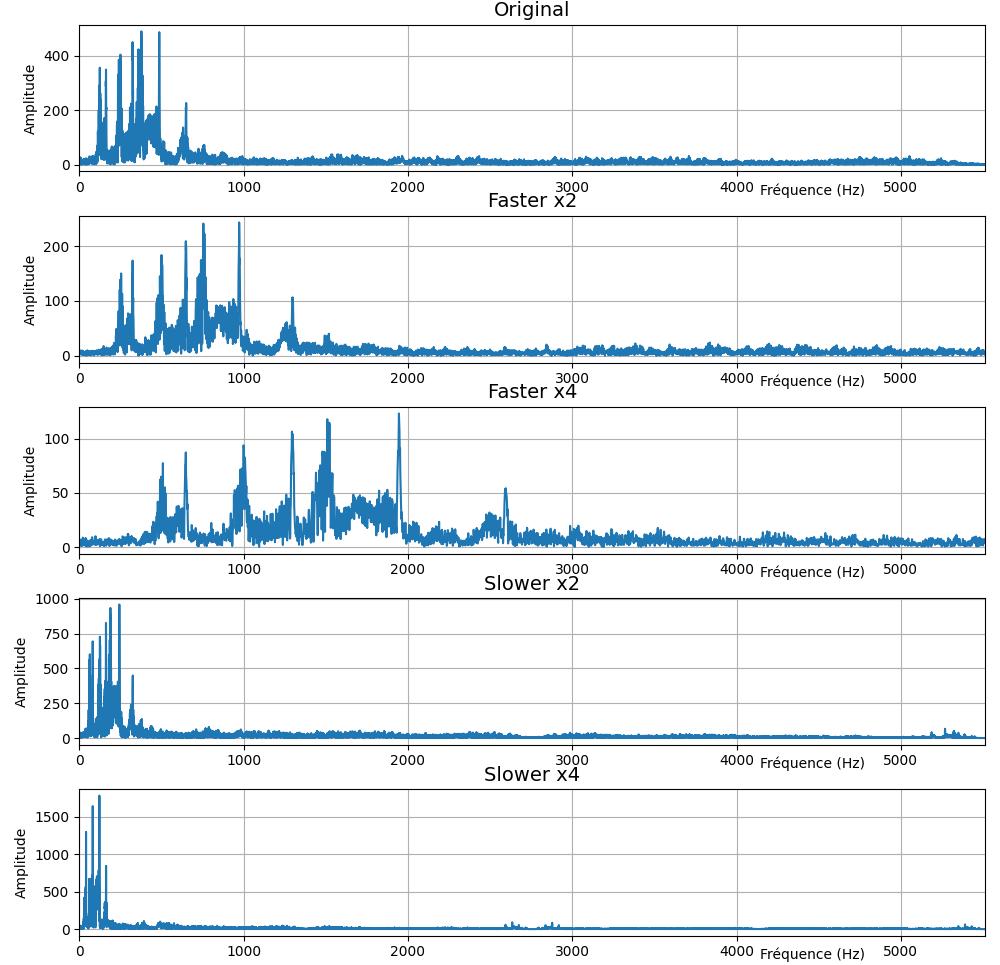
\includegraphics[width=17cm]{screenshots/fft_cadence.png}
    \caption{FFT cadence modifiée}
    \label{fig:cadence_fft}
\end{figure}

Contrairement aux méthodes naïves d’augmentation ou de réduction de cadence par décimation (suppression d’échantillons) ou zéro-padding (ajout de zéros), la fonction \texttt{resample} de SciPy utilise une interpolation efficace basée sur la transformée de Fourier pour reconstruire le signal. Cette approche conserve bien mieux les caractéristiques spectrales du signal, notamment les formants vocaux.

\begin{itemize}
    \item \textbf{À l’écoute}, les signaux transformés avec \texttt{resample} sont plus fluides, plus naturels, et conservent mieux l’intelligibilité du contenu vocal, même pour des facteurs élevés.
    \item En comparaison, la premiére méthode introduit des distorsions, un effet robotique ou haché, et altère la hauteur et le timbre de manière plus brutale.
\end{itemize}

\newpage 
\subsection{Analyse spectrale}
\subsubsection{Analyse d’une tranche de signal par TFD}

\begin{figure}[h!]
    \centering
    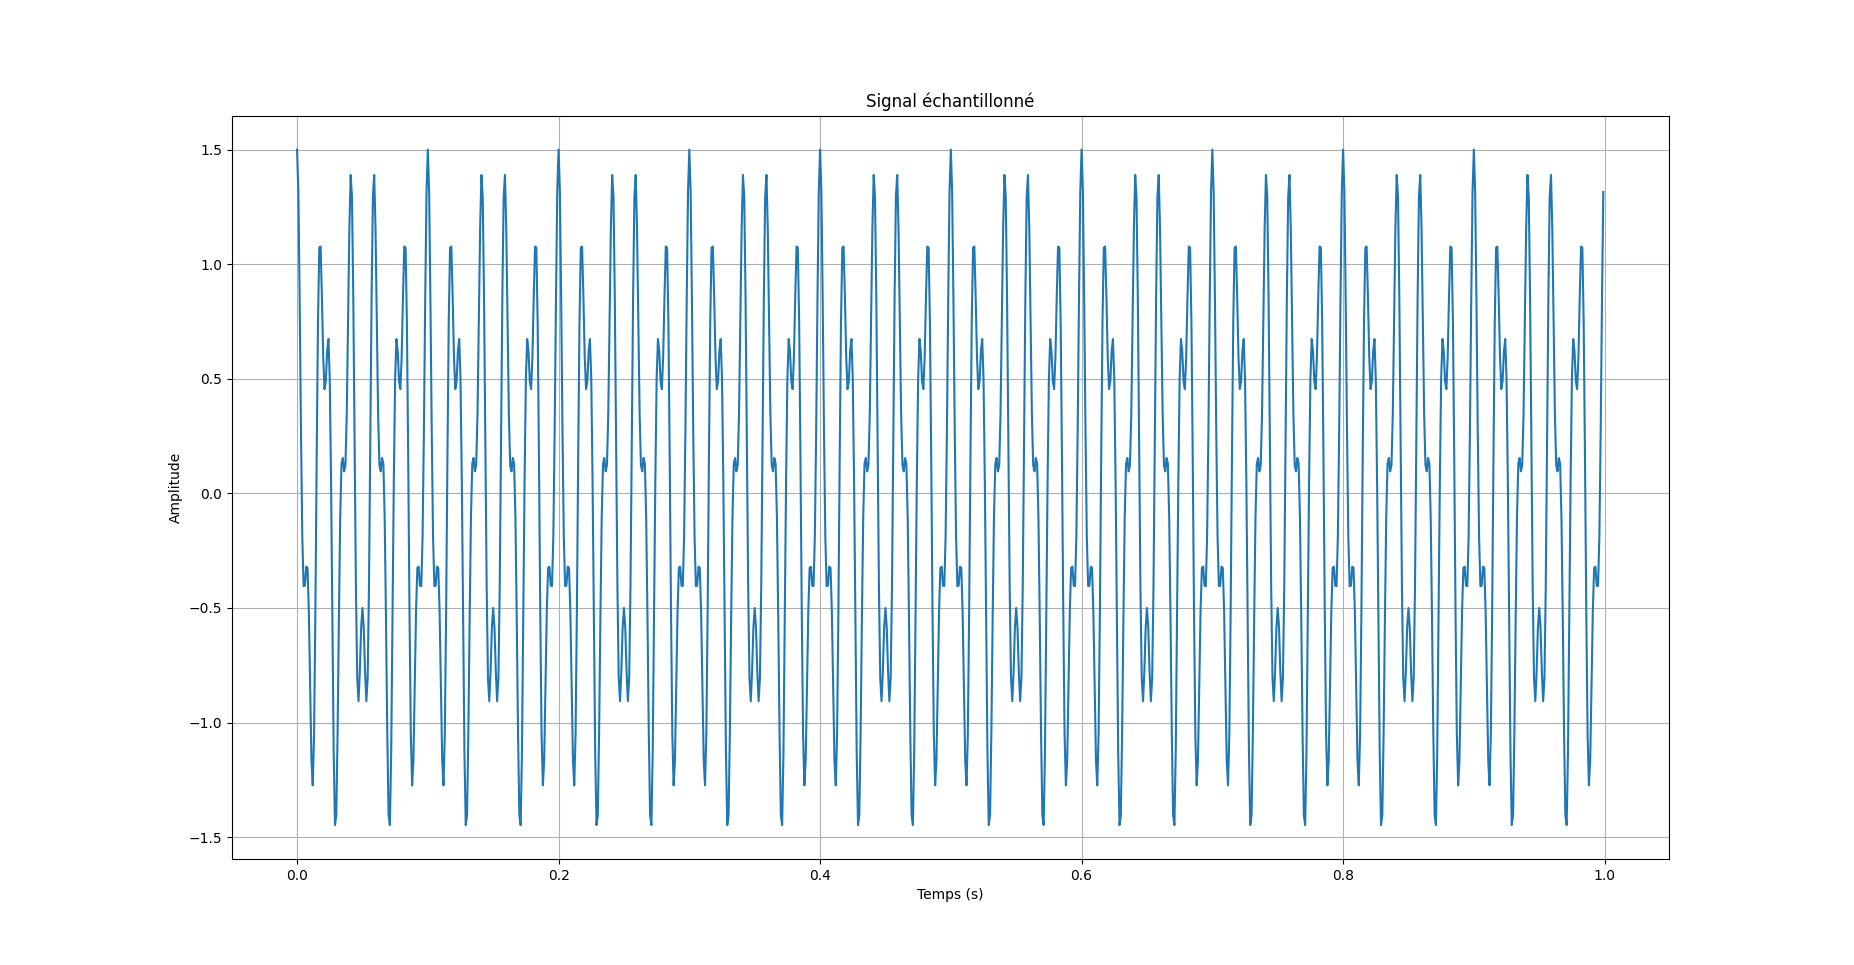
\includegraphics[width=18cm]{screenshots/somme_2_cos.png}
    \caption{exemple d'un signal généré avec: N = 1000 ; fe = 1000 ; f0 = 50 ; f1 = 120 ; A0 = 1.0 ; A1 = 0.5}
\end{figure}

\newpage
La transformée de Fourier discrète d’une fenêtre de Hanning de longueur $N$ présente un module en forme de triangle centré autour de la fréquence zéro. Par analyse expérimentale :

\begin{itemize}
    \item Le lobe principal est bien approximé par une forme triangulaire.
    \item La largeur de ce lobe est d’environ $\frac{4}{N}$ en fréquence normalisée (de $-2/N$ à $+2/N$).
    \item Après normalisation, la surface sous ce lobe principal (approximation de l’intégrale) est proche de 1, ce qui montre que la majorité de l’énergie spectrale est concentrée dans cette bande.
\end{itemize}

Cela justifie l’utilisation fréquente de la fenêtre de Hanning dans les analyses spectrales pour limiter les effets de repliement spectral tout en gardant une bonne localisation fréquentielle.\\

Lorsque la longueur $N$ de la fenêtre de Hanning augmente, on observe que le module de sa transformée de Fourier devient plus "fin". Cela s’explique par le compromis temps–fréquence inhérent à la transformée de Fourier : une plus grande durée d’observation (fenêtre plus longue) permet une meilleure résolution fréquentielle. Ainsi :

\begin{itemize}
    \item Le lobe principal devient plus étroit, avec une largeur approximative de $\frac{4}{N}$.
    \item Le spectre conserve sa forme triangulaire mais est plus concentré autour de la fréquence zéro.
    \item L’amplitude du lobe principal augmente légèrement pour compenser la réduction de largeur (la surface reste $\approx 1$).
\end{itemize}

Cela confirme que la fenêtre de Hanning agit comme un filtre passe-bas doux, et que plus elle est longue, plus elle isole finement une bande de fréquences autour de zéro.

\begin{figure}[h!]
    \centering
    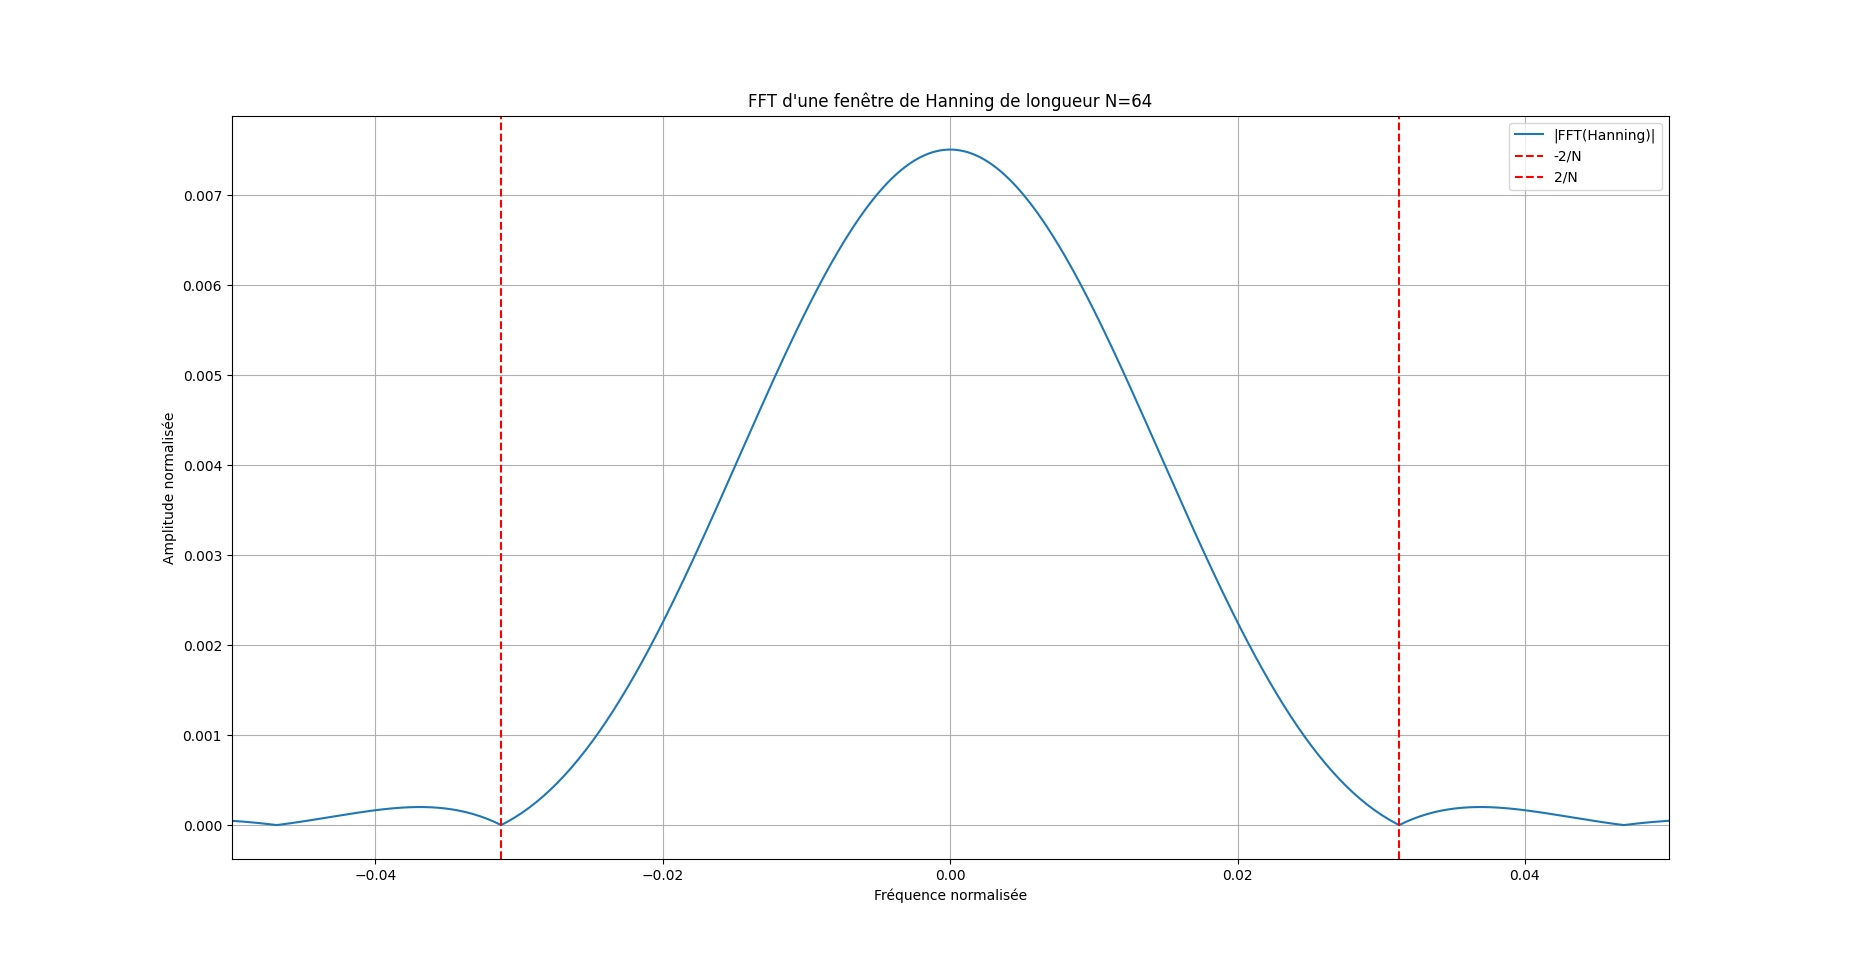
\includegraphics[width=18cm]{screenshots/triangle_hanning.png}
    \caption{FFT fenêtre de Hanning N = 64}
\end{figure}

\begin{figure}[h!]
    \centering
    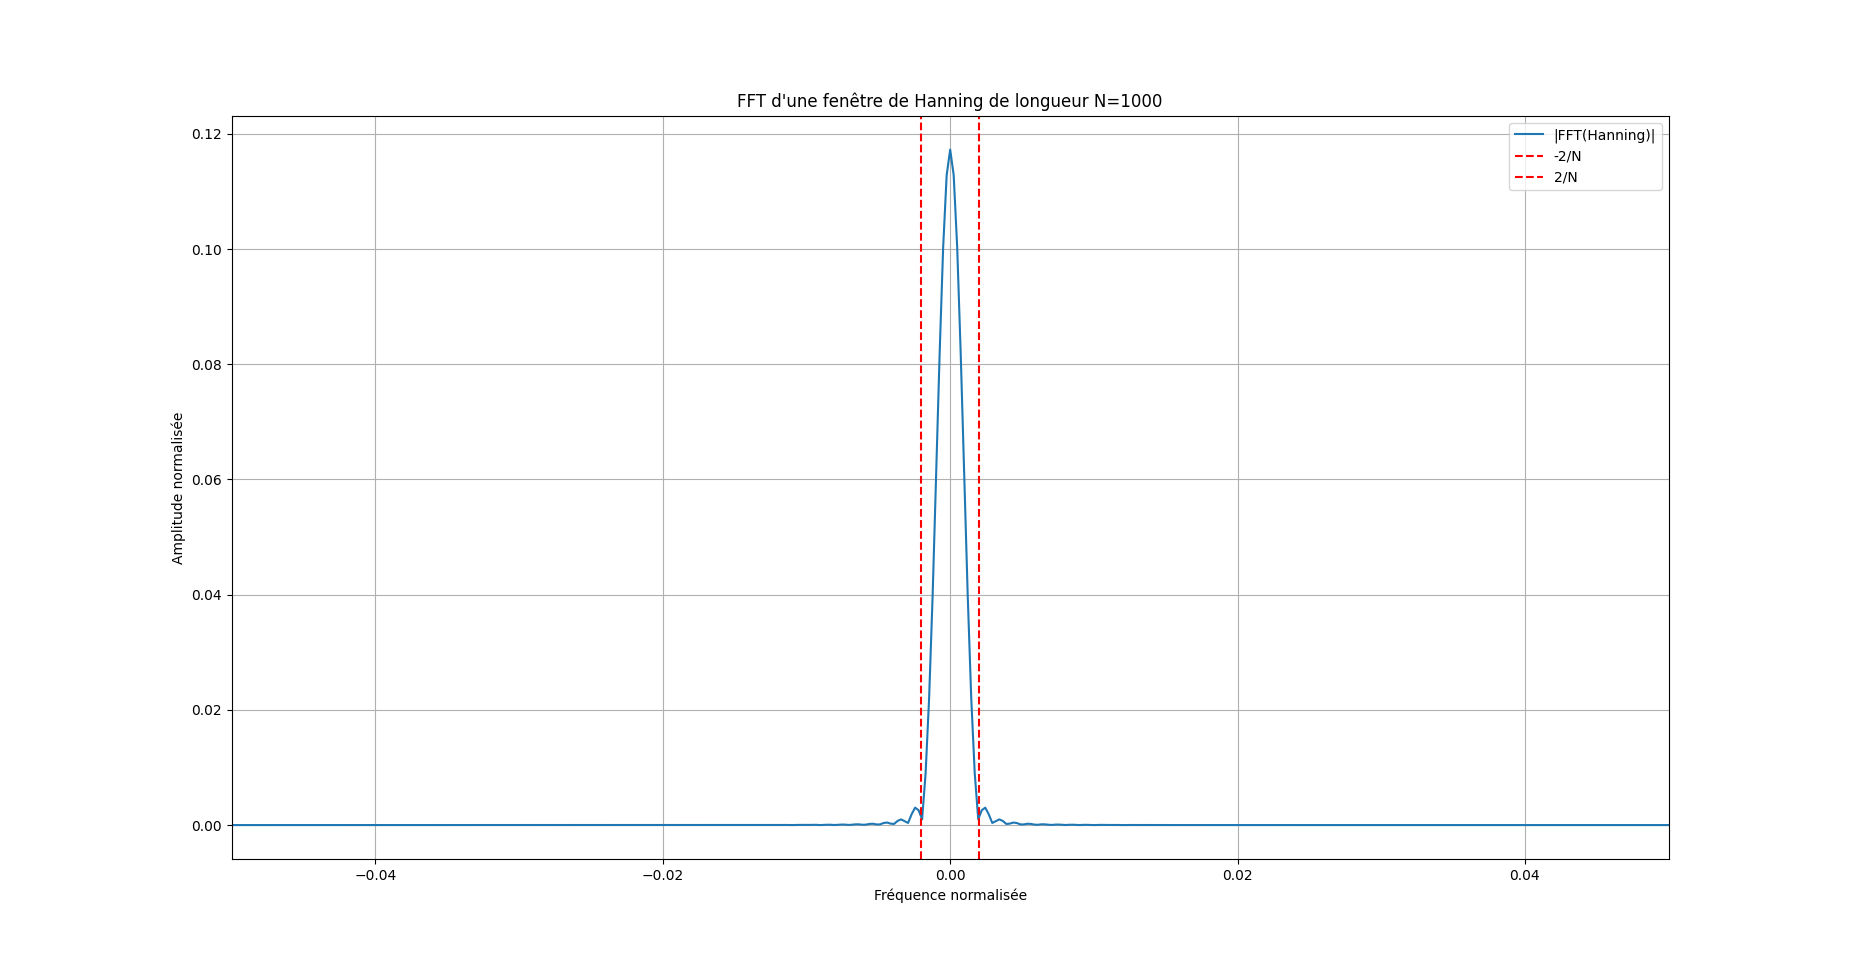
\includegraphics[width=18cm]{screenshots/triangle_hanning_1000.png}
    \caption{FFT fenêtre de Hanning N = 1000}
\end{figure}

\newpage

On considère le signal :
\[
x(t) = A \cos(2\pi f_0 t) + A \cos(2\pi f_1 t)
\]
avec $f_0 = 40~\text{kHz}$, $f_1 = 61~\text{kHz}$, $f_e = 512~\text{kHz}$ et $A = 1$. Le signal est échantillonné et une tranche de $N = 256$ points est extraite pour calculer la TFD après pondération par une fenêtre de Hanning.\\

La transformée de Fourier discrète d’une sinusoïde après pondération par une fenêtre de Hanning est égale à la convolution de la TFD idéale (un pic) avec la TFD de la fenêtre (un triangle de surface unité et de largeur $\frac{4}{N}$).

Chaque sinusoïde donne donc lieu à un lobe triangulaire :

- centré sur $f_0$ et $f_1$ ;\\

- de largeur en fréquence réelle :
\[
\Delta f = \frac{4f_e}{N} = \frac{4 \cdot 512000}{256} = 8000~\text{Hz}
\] \\

Le module de la TFD est donc la somme de deux triangles :\\

- chacun de largeur $8$ kHz (en fréquence) ; \\

- et de surface égale à $1$ (normalisation par la fenêtre).\\

Le spectre montre deux pics nets élargis autour de 40 kHz et 61 kHz, ce qui permet d’estimer les fréquences dominantes du signal malgré la résolution limitée par la fenêtre.\\

La fenêtre de Hanning réduit le leakage spectral (fuites autour des pics), rendant les pics plus nets par rapport à une TFD sans fenêtre.\\

\begin{figure}[h!]
    \centering
    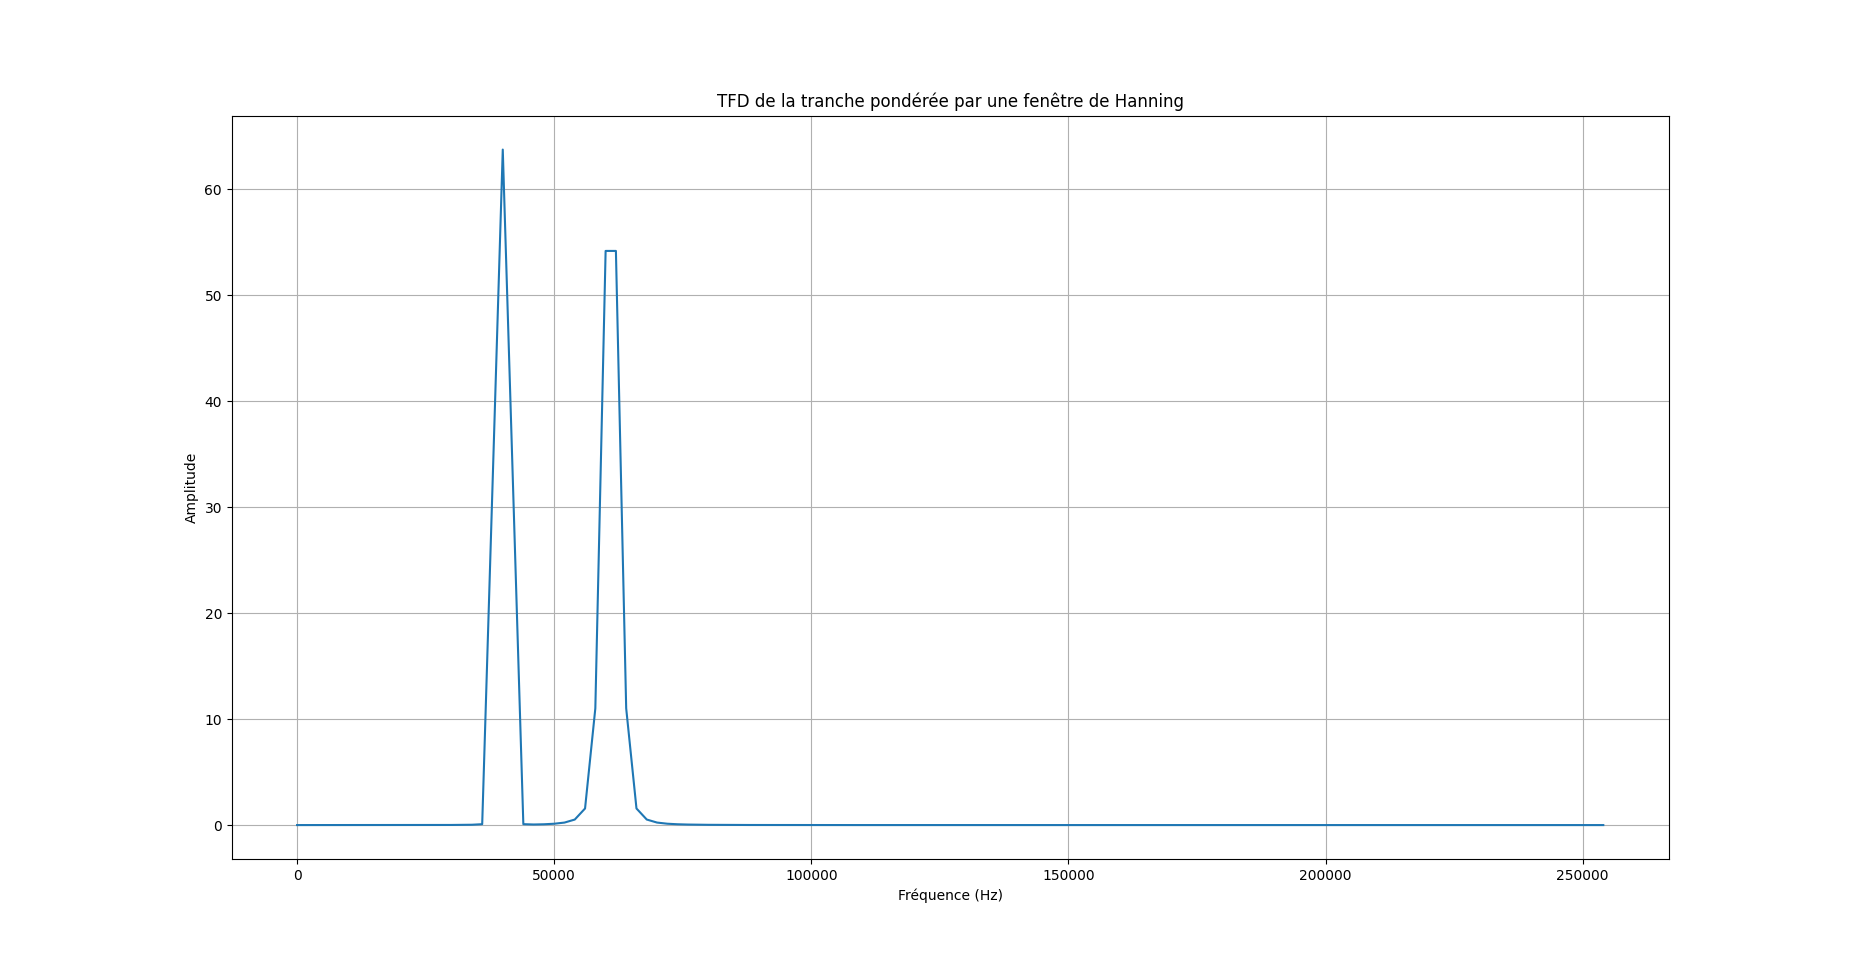
\includegraphics[width=18cm]{screenshots/TFD_hanning_signal.png}
    \caption{TFD avec fenêtre de Hanning}
\end{figure}

\subsubsection{Effets de quelques fenêtres}



